% CREATED BY DAVID FRISK, 2016
\chapter{Experiments}
These experiments are designed to investigate different aspects of information given to the agent, in order to improve performance in the question answering portion of an embodied question answering task. The first experiment investigates how the baseline model is balancing the linguistic and visual information given to it. The second experiment gives the agent categorical information about the things it sees--another type of information about its current location. The third experiment gives the agent new viewpoints during question answering, broadening the visual information the agent has about its current location. The fourth experiment continues to explore the model's balance of common sense and specific knowledge. The fifth experiment combines use of a model pre-trained on another set of images, from another context, with linguistic information in the form of captions to give the agent new information. The sixth experiment investigates if another architecture can give better performance with the available information. 

\todo{add results by question type}
\section{Experiment 1: Baseline and Blindfolding}
\label{sec:exp_1}
\subsection{Method}
The first step was to train and evaluate the baseline that will be used as the point of comparison for all following experiments. This was the CNN and VQA portions of the EQA baseline in habitat-lab, described in~\ref{subsection:model}. A diagram of the VQA model can be seen in Fig.~\ref{fig:baseline_model}. \newline
The next step was to determine if the model was actually considering the visual input when answering questions. This was done via a blindfolding test. There are a number of different ways to conduct blindfolding tests, depending on what you want to test. Because I was interested in if the model was learning visual information during training, I conducted an experiment in which the model was trained normally (the baseline model was used), and then blindfolded only during evaluation. The model was given zeroes instead of the visual content of the scene. This was done by duplicating and modifying the method that converts the .jpgs into numpy arrays to be input to the model, so that it produced an array of zeroes of the same size instead, sending a black/blank image as the input to the model. The point of this blindfolding was to determine if the VQA model was considering the visual input when answering the questions. 
% NI 2021-05-17: here, when you describe how exactly you modified images into empty arrays, you could describe it through formulas, not through text

\begin{figure}[H]
     \centering
     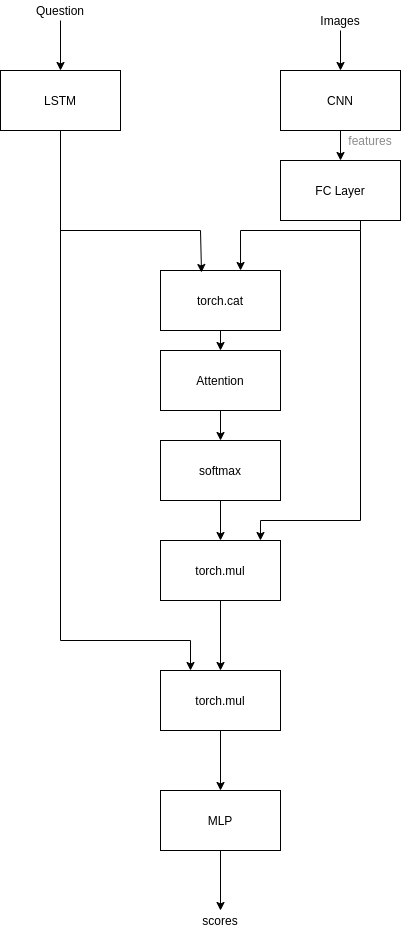
\includegraphics[width=.5\textwidth]{./figure/baseline_diagram.png}
     \caption{VQA Model}
     \label{fig:baseline_model}
\end{figure}

\begin{figure}[H]
	\centering
        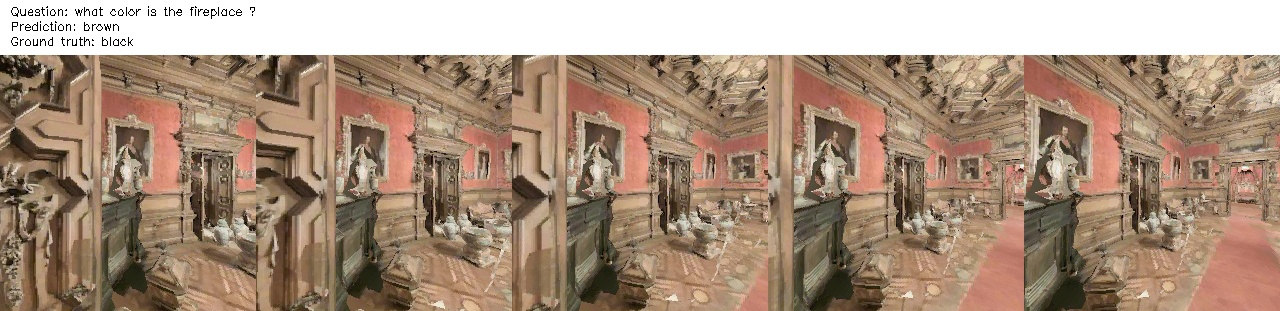
\includegraphics[width=\textwidth]{./figure/results/baseline_and_blindfolding/images/ckpt_23_781_image.jpg}
	\caption{Example VQA Result} % SD 2021-05-01 16:11:24 +0200: You would have to explain in the previous section why we have the input like this. The 5 frames probably means the last five actions taken by the navigation module (and not frames per second in the video sense.)
	\label{fig:example_vqa_result}
\end{figure}

\begin{figure}[H]
	\centering
        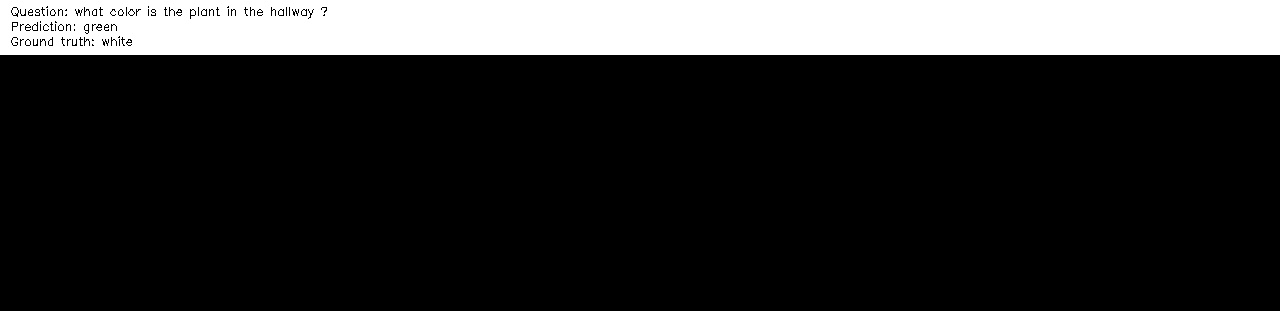
\includegraphics[width=\textwidth]{./figure/results/baseline_and_blindfolding/blindfolded/ckpt_23_1250_image.jpg}
	\caption{Example Blindfolded Result}
	\label{fig:example_blindfolded_result}
\end{figure}
% SD 2021-05-01 15:33:59 +0200: Start with the question first and then describe the exepriment. Discuss also that there are several ways of conducting a blindfold study. For example, the Das et al paper that Nikolai found was changing the architecture of the model and was only using textual information. Why did you choose your method (compared to the other) and what are its implications on results: we test something else, right.

\subsection{Results}
Fig.~\ref{fig:training_metrics} shows metrics for each batch during training, with a weighted average shown in orange. % SD 2021-05-01 15:45:21 +0200: Aha, so the model was trained with vision, just evaluated blindfolded. Cf. Das one could also train it in blindfolded way.
Fig.~\ref{fig:baseline_metrics} shows metrics averaged for each epoch during the baseline evaluation. Fig.~\ref{fig:blindfolded_metrics} shows metrics averaged for each epoch during blindfolded evaluation. It's clear in these graphs that the evaluation results are more stable when the model is given images. As can be seen in Figures~\ref{fig:baseline_loss} \& ~\ref{fig:blindfolded_loss}, the model begins to overfit to the training data around epoch 10.

\begin{figure}[H]
     \centering
     \begin{subfigure}[b]{0.3\textwidth}
         \centering
         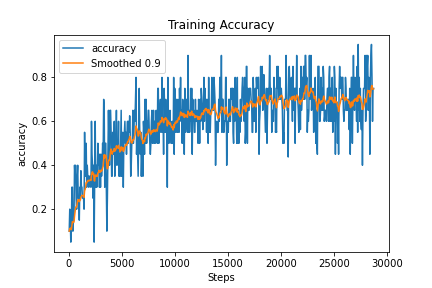
\includegraphics[width=\textwidth]{./figure/results/baseline_and_blindfolding/training/accuracy.png}
         \caption{Accuracy}
         \label{fig:training_accuracy}
     \end{subfigure}
     \hfill
     \begin{subfigure}[b]{0.3\textwidth}
         \centering
         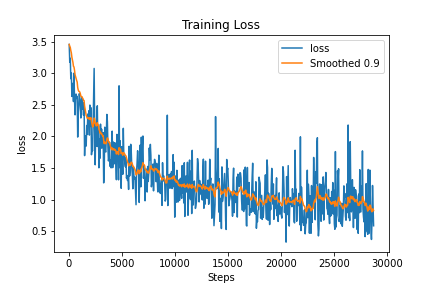
\includegraphics[width=\textwidth]{./figure/results/baseline_and_blindfolding/training/loss.png}
         \caption{Loss}
         \label{fig:training_loss}
     \end{subfigure}
     \hfill
     \begin{subfigure}[b]{0.3\textwidth}
         \centering
         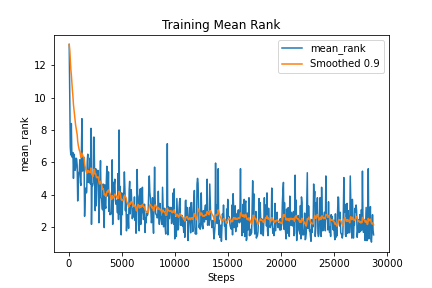
\includegraphics[width=\textwidth]{./figure/results/baseline_and_blindfolding/training/mean_rank.png}
         \caption{Mean Rank}
         \label{fig:training_mean_rank}
     \end{subfigure}
     \caption{Training Metrics}
     \label{fig:training_metrics}
\end{figure}

\begin{figure}[H]
     \centering
     \begin{subfigure}[b]{0.3\textwidth}
         \centering
         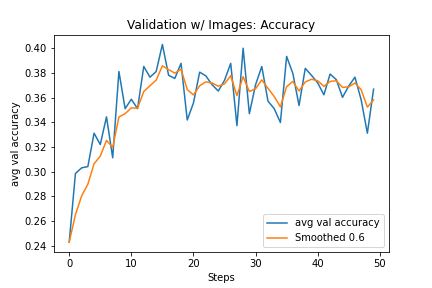
\includegraphics[width=\textwidth]{./figure/results/baseline_and_blindfolding/images/avg val accuracy.png}
         \caption{Accuracy} % SD 2021-05-01 16:14:52 +0200: What is smoothed 0.6?
         \label{fig:baseline_accuracy}
     \end{subfigure}
     \hfill
          \begin{subfigure}[b]{0.3\textwidth}
         \centering
         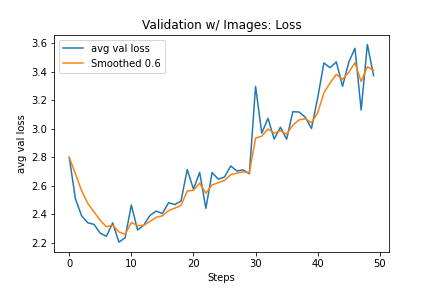
\includegraphics[width=\textwidth]{./figure/results/baseline_and_blindfolding/images/avg val loss.png}
         \caption{Loss}
         \label{fig:baseline_loss}
     \end{subfigure}
     \hfill
     \begin{subfigure}[b]{0.3\textwidth}
         \centering
         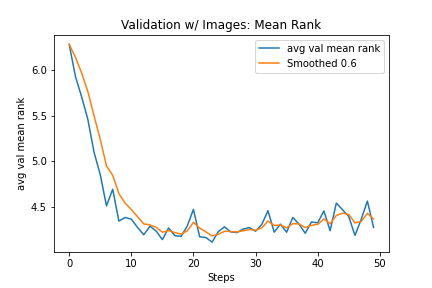
\includegraphics[width=\textwidth]{./figure/results/baseline_and_blindfolding/images/avg val mean rank.png}
         \caption{Mean Rank}
         \label{fig:baseline_mean_rank}
     \end{subfigure}
     \caption{Baseline Evaluation Metrics}
     \label{fig:baseline_metrics}
\end{figure}

\begin{figure}[H]
	\centering
	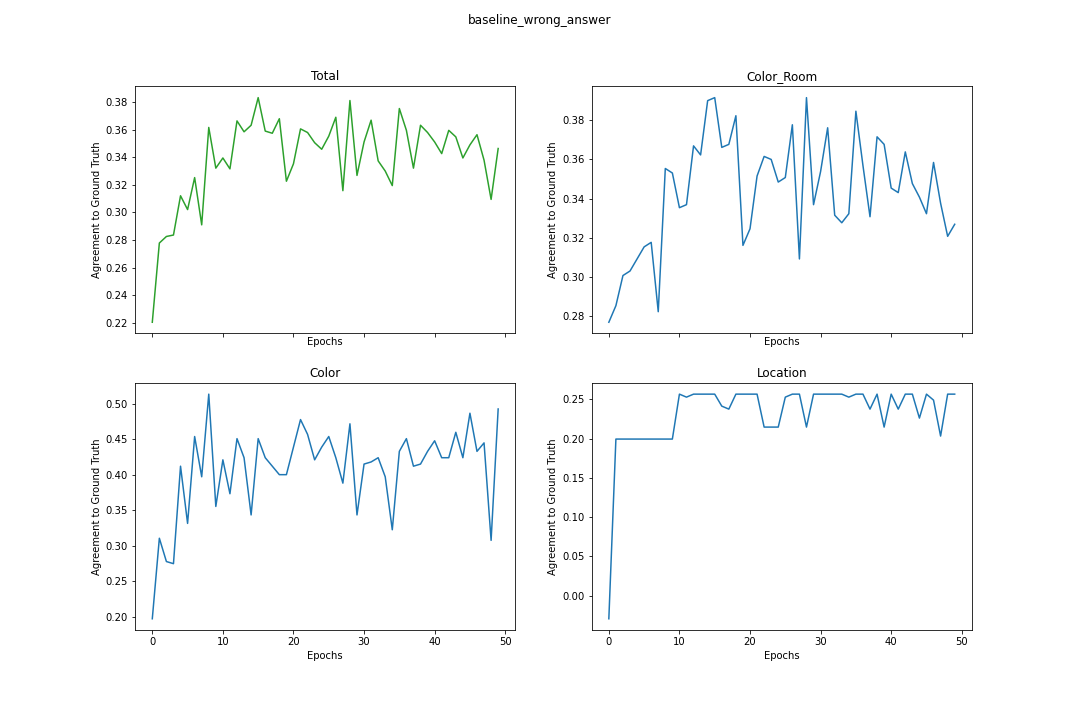
\includegraphics[width=\textwidth]{./figure/wrong_answers/baseline_wrong_answer.png}
	\caption{Baseline: Agreement to Ground Truth by Question Type}
	\label{fig:baseline_agreement}
\end{figure}


\begin{figure}[H]
     \centering
     \begin{subfigure}[b]{0.3\textwidth}
         \centering
         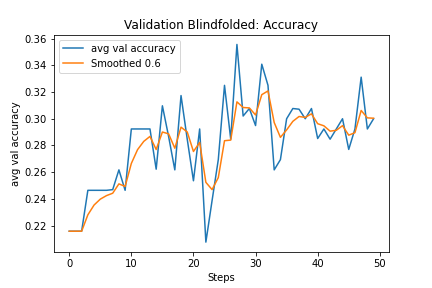
\includegraphics[width=\textwidth]{./figure/results/baseline_and_blindfolding/blindfolded/avg val accuracy.png}
         \caption{Accuracy}
         \label{fig:blindfolded_accuracy}
     \end{subfigure}
     \hfill
     \begin{subfigure}[b]{0.3\textwidth}
         \centering
         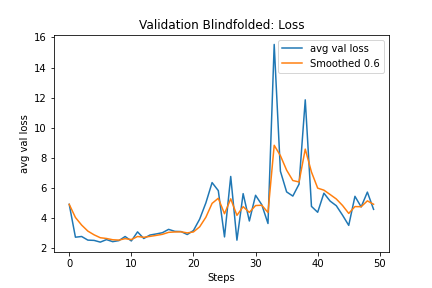
\includegraphics[width=\textwidth]{./figure/results/baseline_and_blindfolding/blindfolded/avg val loss.png}
         \caption{Loss}
         \label{fig:blindfolded_loss}
     \end{subfigure}
     \hfill
     \begin{subfigure}[b]{0.3\textwidth}
         \centering
         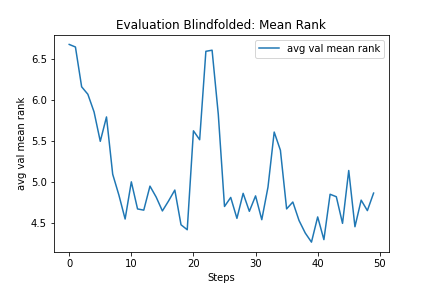
\includegraphics[width=\textwidth]{./figure/results/baseline_and_blindfolding/blindfolded/avg val mean rank.png}
         \caption{Mean Rank}
         \label{fig:blindfolded_mean_rank}
     \end{subfigure}
     \caption{Blindfolded Evaluation Metrics}
     \label{fig:blindfolded_metrics}
\end{figure}
% SD 2021-05-01 15:48:38 +0200: I assume validation is performed after training each epoch. The model shows that a blindfolded model is more confused even during training which we can accept since the model is not really optimised on a blindfolded scenario. It would be interesting to see what would happen if the model is optimised on black images. Hence, you analysis raises new questions which would be interisting to answer. However, for the original question it would just be enough to report the final mean rank on the test set.
Table~\ref{tab:best_baseline} shows the checkpoints with lowest loss, highest accuracy, and lowest mean rank during the evaluation of the baseline, with the metric that was "best" during that checkpoint in bold. Table~\ref{tab:best_blindfolded} shows the same for blindfolded evaluation. Comparing their best, the blindfolded model has 4.7\% worse accuracy than the baseline and 0.149 higher mean rank. These are also not achieved at the same checkpoint--the best model to use with visual input is the not the one that works best when forced to rely entirely on linguistic input. \newline % SD 2021-05-01 15:57:27 +0200: But of course the points at which this was achieved are different. Hence, the best model that we produce using images is not the best model to work in a blindfolded scenario.
\begin{table}[H]
\centering
\caption{"Best" Epochs During Baseline Evaluation}
\begin{tabular}{l | l | l | l}
Checkpoint & Loss & Accuracy & Mean Rank \\
\hline
8 & \textbf{2.204141} & 0.381122 & 4.341837 \\
15 & 2.404433 & \textbf{0.403061} & 4.138265 \\
23 & 2.691763 & 0.370408 & \textbf{4.110714}
\end{tabular}
\label{tab:best_baseline}
\end{table}

\begin{table}[H]
\centering
\caption{"Best" Epochs During Blindfolded Evaluation}
\begin{tabular}{l | l | l | l}
Checkpoint & Loss & Accuracy & Mean Rank \\
\hline
5 & \textbf{2.416477} & 0.246429 & 5.493877 \\
27 & 2.546098 & \textbf{0.355612} & 4.551021 \\
39 & 4.788071 & 0.307653 & \textbf{4.260204}
\end{tabular}
\label{tab:best_blindfolded}
\end{table}

One question here is whether the blank inputs to the model are actively confusing it--in training it is always given an image, so this black input is a completely new case. This could also explain the differences to a previous student's course project, in which they found equivalent performance to baseline when the agent was given a random image from the dataset. One challenge here is that scenes are used for multiple questions, % SD 2021-05-01 15:59:17 +0200: the model might be getting the correct answers by chance. If we measure accuracy then we could integrate agreement by chance using the Kappa co-efficient: http://cswww.essex.ac.uk/technical-reports/2005/csm-437.pdf
so this leaves open the possibility that the item being asked about is actually present in the room. Even using scenes not included in the dataset would be difficult to control, since if you ask the agent 'what color is the bookshelf?', you would then need to confirm that no bookshelves are present in the random image. \newline

% SD 2021-05-01 16:03:30 +0200: There are a lot of questions that are interesting (and open) in this section, we could do more experiments and also there are diferent ways at looking at results. The focus on epochs shows how confused is your model during training when evaluated by blindfolded images. It is also interesting that the model gets more confused in later epochs, perhpas important vision information is only learned then? But how confused would be the best model that would be selected in training if blindfolded? What happens if we train the model blindfolded? We could therefore expand the discussion here significantly.


\section{Experiment 2: Basic Semantic Categories}
\label{sec:exp_2}
\subsection{Method}
Schüz and Zarrieß found that models with prior knowledge about objects were able to make better predictions about those objects, and they found that an 'Early Fusion' strategy of integrating the object type information allowed the model to make better predictions about atypical colors of common objects\cite{colorknowledge}. Since one of the concerns with EQA models is that they are relying too heavily on common sense knowledge of objects, this is exactly what we would like to achieve--improving predictions about specific objects, which, if the prior knowledge about colors is not correct for the object, may be of atypical color. Based on this, I combined category information about objects in the scene with the visual features before attending with the question, as shown in Fig.~\ref{fig:category_model}. The categorical information comes from the 'semantic sensor' of the agent in habitat-sim, which reads annotations from the dataset. It reads annotations of object instances, which can then be mapped to category ids. The list of category IDs can be found in appendix~\ref{app:categories}.
\todo{Discuss shaping!}

% SD 2021-05-01 15:37:23 +0200: Why do we believe semantic segmentation will be helpful? Also, point out that the categories for semantic segmentations are just general labels for surfaces and objects and than QA on object requires more detailed semantic information about the objects, including common sense knowledge that you mentioned earlier. Why place semantic segmentation after the linguistic and perceptual attention? What are our hypotheses?
\begin{figure}[h]
     \centering
     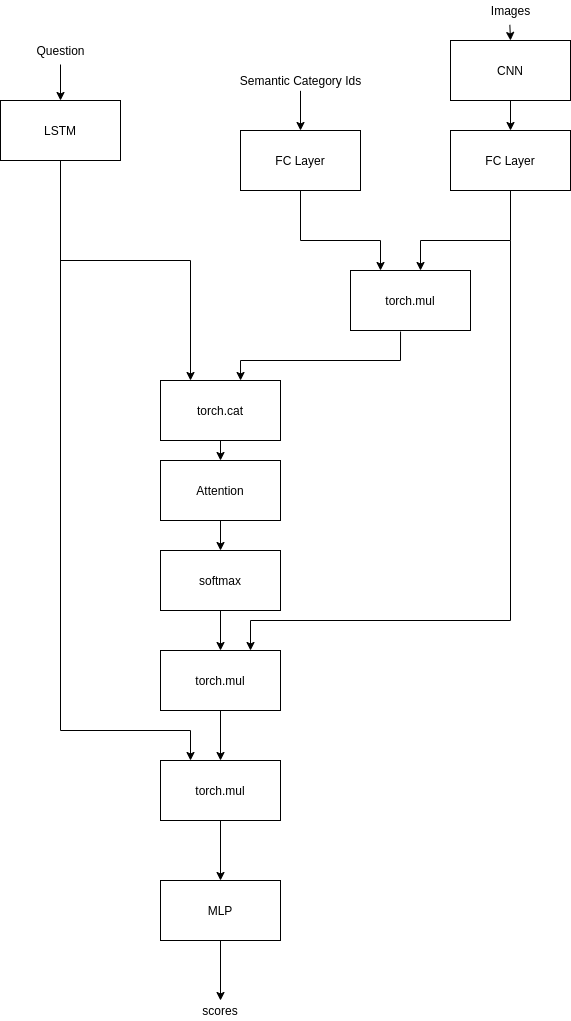
\includegraphics[width=.75\textwidth]{./figure/model_w_semantic.png}
     \caption{Model With Semantic Category IDs as 3rd input}
     \label{fig:category_model}
\end{figure}

\subsection{Results}
In this experiment, the model was provided with semantic category information, as described above.
With the categories, the highest accuracy on the evaluation set was 1.4\% higher than the baseline's highest accuracy, and the highest mean rank was 0.46 higher than the baseline's highest. 

% SD 2021-05-01 16:16:09 +0200: Note that since you are using a different model now the loss here is not comprabale with the loss of the previous baseline model. We need to find a way to demonstrate the improvement (or no improvement): the final mean rank on the test set?

\begin{figure}[H]
     \centering
     \begin{subfigure}[b]{0.4\textwidth}
         \centering
         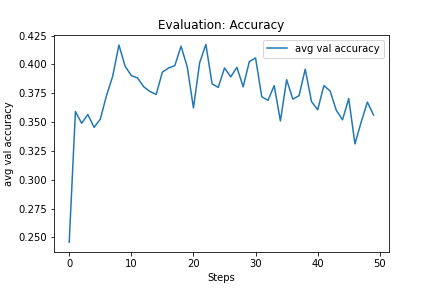
\includegraphics[width=\textwidth]{./figure/results/semantic_categories/eval/avg val accuracy.png}
         \caption{Accuracy}
         \label{fig:category_accuracy}
     \end{subfigure}
     \hfill
     \begin{subfigure}[b]{0.4\textwidth}
         \centering
         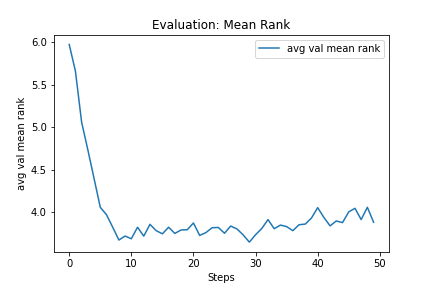
\includegraphics[width=\textwidth]{./figure/results/semantic_categories/eval/avg val mean rank.png}
         \caption{Mean Rank}
         \label{fig:category_mean_rank}
     \end{subfigure}
     \caption{Evaluation Metrics for model given semantic categories}
     \label{fig:category_metrics}
\end{figure}

\begin{table}[H]
\centering
\caption{"Best" Epochs During Evaluation of Model with Semantic Categories}
\begin{tabular}{l | l | l | l}
Checkpoint & Loss & Accuracy & Mean Rank \\
\hline
6 & \textbf{2.108628} & 0.372959 & 3.971939 \\
22 & 2.444937 & \textbf{0.417347} & 3.761735 \\
29 & 2.824962 & 0.402551 & \textbf{3.650510} 
\end{tabular}
\label{tab:best_category}
\end{table}

\section{Experiment 3: Look Around}
\label{sec:exp_3}
\subsection{Method}
This experiment attempts to increase the usefulness of the visual information being provided to the model. The VQA model takes in the last five frames of navigation as its visual input. However, as seen in Fig.~\ref{fig:example_vqa_result}, these images are very similar to each other, and often have odd angles of the object in consideration. This experiment implements a look around procedure, where the agent takes a series of moves (look left, look right, etc) at the end of navigation, so that the last five frames give more varied viewpoints of the room and object. The hypothesis here was that the model should, given the larger visual context, perform better on location questions. \newline
The 'frame queues' for each episode are generated before beginning training or evaluation, by saving the rgb observations of the agent at specified positions and rotations. (These are given in a global coordinate frame.) In the baseline model, this frame queue is that last five frames of navigation. For the look around experiment, this queue is: the final position and rotation of navigation, a frame from the same position turned 0.523599 radians to the left, same position turned 0.523599 radians to the right (from the original rotation), same position turned up 0.2617995 radians (from the original rotation), and the same position turned down 0.2617995 radians (from the original rotation). As can be seen in Fig.~\ref{fig:look_around}, this gives more variation in the final five frames. \newline
Rotations are represented as quaternions, a compact representation that doesn't suffer from gimbal lock. These quaternions are expressed in [x, y, z, w]. The new rotations are calculated by: \\ \begin{math}
original = [x0, y0, z0, w0] \\
rotate = [0, 1, 0, rotation\_amount] \\
new\_quaternion = original * rotation
\end{math}

\begin{figure}[H]
	\centering
	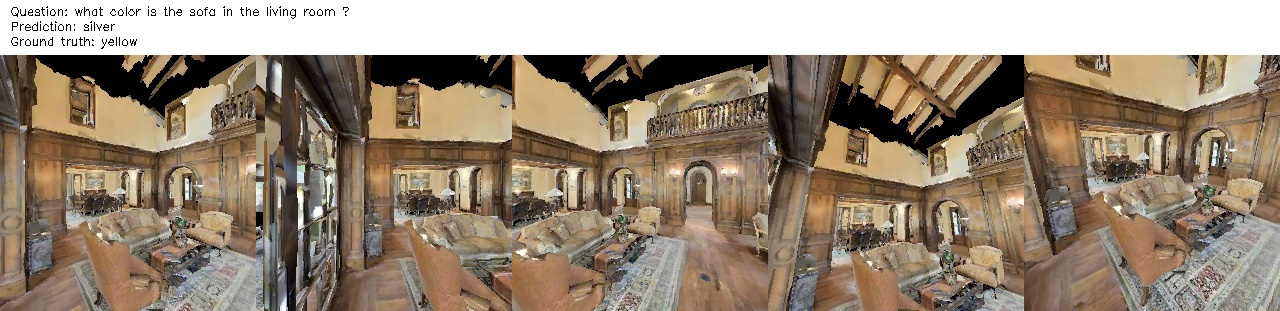
\includegraphics[width=\textwidth]{./figure/lookaroundexample.jpg}
	\caption{Look Around Example}
	\label{fig:look_around}
\end{figure}

\todo{discuss new versions of look around}
% NI 2021-05-17: we should cover/mention that a different (but related) experiment could be to start look around not near the object, but some time before it reaches the object. can be a possible solution to 'these images are very similar to each other, and often have odd angles of the object in consideration'?

\subsection{Results}
Using Look Around, the model was able to perform slightly better than baseline. The best mean rank was 0.41 lower than baseline, and the highest accuracy was 0.9\% higher than baseline. 
\begin{figure}[H]
     \centering
     \begin{subfigure}[b]{0.3\textwidth}
         \centering
         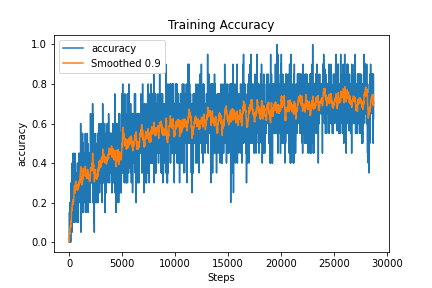
\includegraphics[width=\textwidth]{./figure/results/look_around/training/accuracy.png}
         \caption{Training Accuracy}
         \label{fig:la_t_accuracy}
     \end{subfigure}
     \hfill
     \begin{subfigure}[b]{0.3\textwidth}
         \centering
         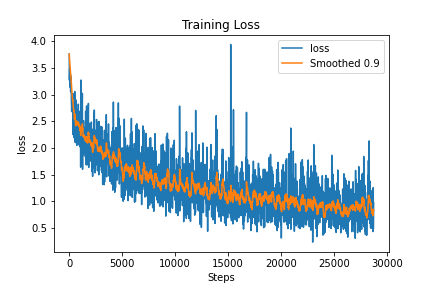
\includegraphics[width=\textwidth]{./figure/results/look_around/training/loss.png}
         \caption{Training Loss}
         \label{fig:la_t_loss}
     \end{subfigure}
     \hfill
     \begin{subfigure}[b]{0.3\textwidth}
         \centering
         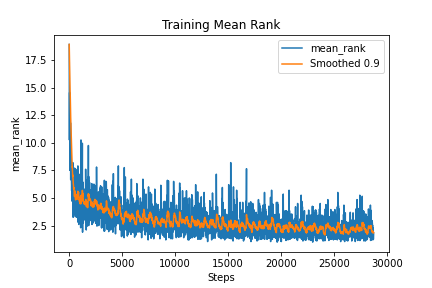
\includegraphics[width=\textwidth]{./figure/results/look_around/training/mean_rank.png}
         \caption{Mean Rank}
         \label{fig:la_t_mean_rank}
     \end{subfigure}
     \caption{Look Around Training Metrics}
     \label{fig:la_t_metrics}
\end{figure}

\begin{figure}[H]
     \centering
     \begin{subfigure}[b]{0.3\textwidth}
         \centering
         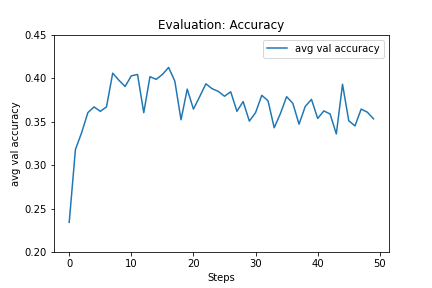
\includegraphics[width=\textwidth]{./figure/results/look_around/eval/avg val accuracy.png}
         \caption{Accuracy}
         \label{fig:la_e_accuracy}
     \end{subfigure}
     \hfill
     \begin{subfigure}[b]{0.3\textwidth}
         \centering
         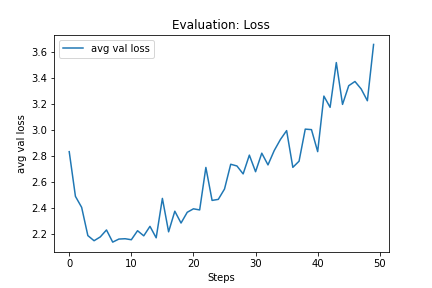
\includegraphics[width=\textwidth]{./figure/results/look_around/eval/avg val loss.png}
         \caption{Loss}
         \label{fig:la_e_loss}
     \end{subfigure}
     \hfill
     \begin{subfigure}[b]{0.3\textwidth}
         \centering
         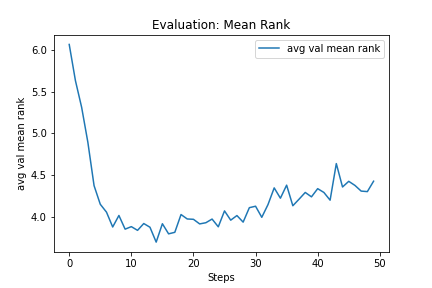
\includegraphics[width=\textwidth]{./figure/results/look_around/eval/avg val mean rank.png}
         \caption{Mean Rank}
         \label{fig:la_e_mean_rank}
     \end{subfigure}
     \caption{Look Around Evaluation Metrics}
     \label{fig:la_e_metrics}
\end{figure}

\begin{table}[H]
\centering
\caption{"Best" Epochs During Evaluation of Model using Look Around (30, 30, 15, 15)}
\begin{tabular}{l | l | l | l}
Checkpoint & Loss & Accuracy & Mean Rank \\
\hline
7 & \textbf{2.140735} & 0.405612 & 3.881122 \\
16 & 2.219612 & \textbf{0.412245} & 3.798980 \\
14 & 2.173734 & 0.398469 & \textbf{3.700000} 
\end{tabular}
\label{tab:best_look_around}
\end{table}

\section{Experiment 4: Blind}
\label{sec:exp_4}
\subsection{Method}
For this experiment, the same function used to blindfold the model in Experiment 1 was also applied during training. This was done in order to have a 'text-only' baseline without changing the architecture of the model, and to attempt to address the question of how much the model was being confused by the 'new' case of a black image after training with normal images during Experiment 1. 

\subsection{Results}
The model trained without images, at its best checkpoints, performed comparably to the model trained with images and then blindfolded later, however, there is a clearer trajectory of the behaviour from checkpoint to checkpoint, as seen comparing Fig.~\ref{fig:fb_e_metrics} and Fig.~\ref{fig:blindfolded_metrics}.

\begin{figure}[H]
     \centering
     \begin{subfigure}[b]{0.3\textwidth}
         \centering
         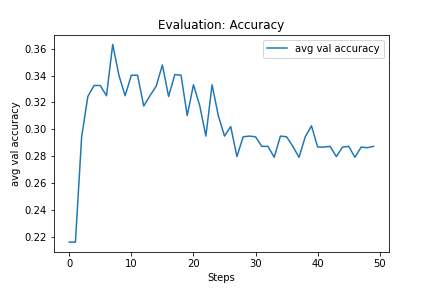
\includegraphics[width=\textwidth]{./figure/results/fully_blinded/eval/avg val accuracy.png}
         \caption{Accuracy}
         \label{fig:fb_e_accuracy}
     \end{subfigure}
     \hfill
     \begin{subfigure}[b]{0.3\textwidth}
         \centering
         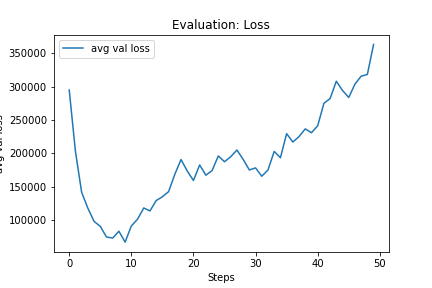
\includegraphics[width=\textwidth]{./figure/results/fully_blinded/eval/avg val loss.png}
         \caption{Loss}
         \label{fig:fb_e_loss}
     \end{subfigure}
     \hfill
     \begin{subfigure}[b]{0.3\textwidth}
         \centering
         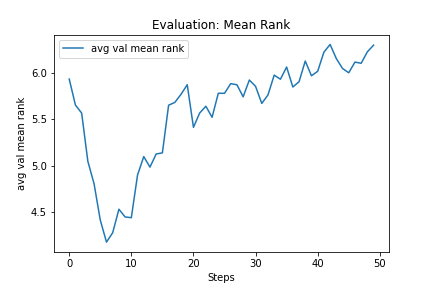
\includegraphics[width=\textwidth]{./figure/results/fully_blinded/eval/avg val mean rank.png}
         \caption{Mean Rank}
         \label{fig:fb_e_mean_rank}
     \end{subfigure}
     \caption{Fully Blinded Evaluation Metrics}
     \label{fig:fb_e_metrics}
\end{figure}

\begin{table}[H]
\centering
\caption{"Best" Epochs of Blind Model}
\begin{tabular}{l | l | l | l}
Checkpoint & Loss & Accuracy & Mean Rank \\
\hline
7 & 73306.476562 & \textbf{0.363265} & 4.273469 \\
6 & 74890.796875 & 0.325000 & \textbf{4.171429}
\end{tabular}
\label{tab:best_blind}
\end{table}

\section{Experiment 5: Dataset Boosting}
\label{sec:exp_5}
\subsection{Method}
\todo{performance between question types, scikit learn boosting}

\subsection{Results}

